% !TEX root = ../../../main.tex
% 来源：中学数学实验教材·第三册（高中数学）
% 章节：任意角的三角函数 / 三角函数的诱导公式
% 原始文件：6.tex，行 1944-1955
% 类型：tikz
% ---
    \begin{tikzpicture}[>=latex, scale=1]
        \draw[<->] (-0.75,0)--node[fill=white]{$\tfrac{\sqrt{3}}{2}$}(-.75,.75*1.732);
    \draw[->](-2,0)--(2.5,0)node[right]{$x$};
    \draw[->](0,-2)--(0,2.5)node[right]{$y$};
    \draw (0,0) circle(1.5);   
    \node at (-.25,-.25){$O$};
    \draw[very thick](0,0)--(1.5/2,1.5/2*1.732)node[right]{$P_1$}--(-1.5/2,1.5/2*1.732)node[left]{$P_2$}--(0,0);
    \draw[->](.5,0) arc (0:60:.5);
    \node at (30:.7){$\frac{\pi}{3}$};
    \node at (2,0)[below]{$A(1,0)$};

    \end{tikzpicture}
